\chapter{OpenShift容器云平台和MRWS实验测试}
提出MRWS调度方案优化OpenShift容器云平台底层容器编排引擎Kubernetes调度流程和调度算法后,需要对其资源利用率和负载均衡性进行评估测试。本章主要实验包括如下几个部分:
\begin{enumerate}[(1)]
	\item 在ContainerCloudSim容器云仿真平台上进行大规模容器应用仿真调度实验、对比Kubernetes默认算法、Random算法和MRWS调度算法在资源利用率和负载均衡性方面的性能。
	\item 基于开源OpenShift Origin搭建开发了Paladin容器云平台,该平台是一个集海量数据存储管理、多计算框架快速部署、调度优化、用户注册、按需服务等多功能的容器云PaaS平台。
	\item 在Paladin开发多种分布式计算框架,将其打包成镜像文件,存储在镜像仓库汇中,用户可以快速构建开发测试环境。
	\item 在Paladin平台上开发MRWS算法的调度器,使用多中计算框架容器应用混合部署测试其性能,并与其他调度算法进行对比。
\end{enumerate}

\section{ContainerCloudSim模拟MRWS调度方案}
实验室基于开源OpenShift Origin开发的容器云PaaS平台是在小规模实际物理机上部署,不能进行调度方案的大规模测试和分析,为了评估方案的性能和可靠性,首先在容器云仿真平台ContainerCloudSim上进行大规模的仿真实验。首先构建仿真实验环境,然后开发Kubernetes默认Default调度算法、Random和MRWS调度算法,使用大规模负载进行测试分析。

\subsection{ContainerCloudSim容器云仿真平台}
\subsubsection{CloudSim云仿真平台}
容器和容器编排技术的逐渐成熟推动了容器云的飞速发展,在计算中心的容器云上为了评测资源调度策略和容器服务性能,一个容器云仿真平台变得异常重要。经过大量测试对比调度方案,不仅可以节约开发时间,也能避免造成资源浪费和减少试错成本。针对每一个调度方案,如果部署大规模容器云平台进行性能分析测试,绝大多数的小公司和开发人员并不具备这种条件。在传统的云计算模式下,应用服务的组成、供应、配置和部署条件较为复杂,当用户需求和系统配置动态变化时,评估一个调度策略以及工作负载是相当困难的,一个优秀的云计算平台模拟器可以很好解决这个问题。一个云平台模拟器通过控制环境变量和重复试验可以加速理论研究和开发过程,根据需求和应用场景不同,各大公司和研究机构推出了一系列的云计算平台仿真工具。

MDCSim是一个全面、灵活、可扩展的多层数据中心模拟器,整个模拟平台分为通信层、内核层和用户层建模,通信层用于模拟模拟集群内部通信、内核层模拟调度和分析系统性能、用户层用于模拟各种应用。该模拟器可以根据底层不同硬件特点进行混合建模,用于评估数据中心的能耗,让用户在保持低功耗的同时实现集群服务性能的提升。GroudSim是一个基于Java的模拟器,用于模拟科学应用在网格和云设施上执行问题,模拟完成后给用户提供了基础的统计和分析功能。NetworkCloudSim用于解决网络模拟问题,弥补其他模拟器对网络细节关注不足,支持MPI和工作流。TeachCloud用于对MapReduce应用建模并集成一个负载生成器,提供图形化的接口和实现定制的网络拓扑结构。CloudSim是墨尔本大学Gridbus项目推出的云计算仿真软件,既能对系统性能和应用服务模拟、仿真、试验,也能评估资源调度策略的优劣。

CloudSim是一个开源的仿真软件,最大特点就是提供一个虚拟化引擎,帮助数据中心建立和管理各种虚拟化服务。支持大规模云计算资源管理和调度模拟,将数据中心的资源虚拟化为资源池,CloudSim的分层体系架构图如5.1所示。
\begin{figure}[H] % use float package if you want it here
	\centering
	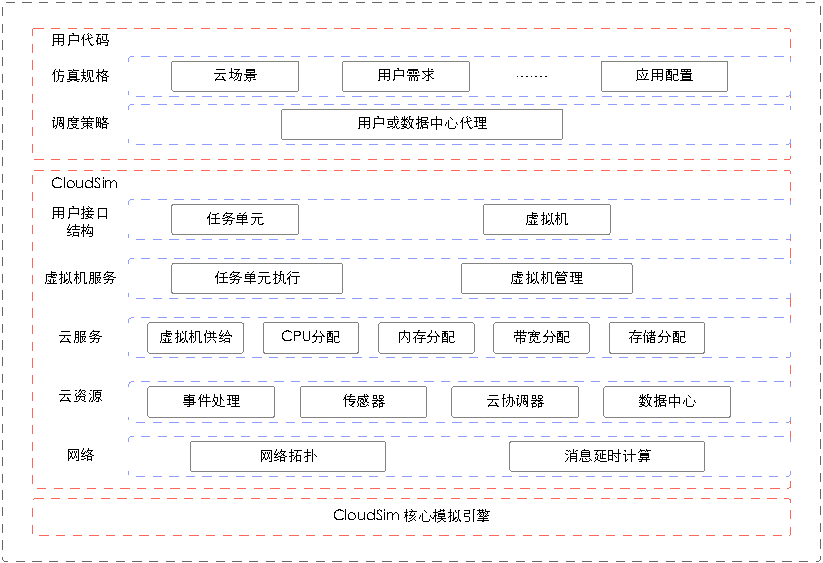
\includegraphics{cloudsim-layer}
	\caption{CloudSim分层架构图}
	\label{fig:xfig1}
\end{figure}

CloudSim是一个分层构建的体系结构,从下到上一次为CloudSim核心引擎层、网络、云资源、云服务、虚拟服务、用户接口结构、资源调度以及仿真规格层。下面一次介绍各层次的大致作用:
\begin{enumerate}[(1).]
	\item CloudSim核心引擎层是离散数据模拟引擎SimJava,为上层提供系统组件构建如服务、数据中心、客户端、代理、虚拟机等,查询和时间处理、通信、模拟时钟等功能。
	\item Network层模拟网络组件如资源收集、数据集、负载测试、信息服务等,对网络设施建模,支持高层软件组件。
	\item 云资源层主要是Host主机和数据中心,主机的核心硬件设施通过数据中心类建模,处理服务请求,构成虚拟资源池。
	\item 云服务层给客户端分配特定应用的VM,同时给VM分配处理内核、内存、磁盘以及网络带宽,可以执行用户新的VM提供策略,有助于一定目标优化。
	\item 虚拟机服务层提供任务执行和虚拟机管理,定义一系列虚拟机创建、销毁、合并、迁移等操作管理,执行基于云环境的应用服务。
	\item 用户接口层向用户提供VM任务单元和虚拟机,将下层的虚拟资源打包成虚拟机提供给用户。
	\item 用户代码层是用户根据实际应用场景和需求,定制应用的规格和调度策略,将应用加入数据中心的代理中,按照资源调度策略进行调度。
\end{enumerate}
CloudSim有一些重要的类和核心概念,针对这些类的大致作用进行简单的介绍:
\begin{enumerate}[1.]
	\item DataCenter类封装底层的Host主机,提供虚拟化的资源,保证每个数据中心至少存在一台运行的Host主机,同时提供虚拟化网络并内置了一个调度组件,为虚拟机和主机分配CPU、内存、网络带宽等资源。
	\item DataCenterBroker类是数据中心代理,负责虚拟机和云任务列表的提交。
	\item VM类是虚拟机类,运行在Host上,多个VM共享Host资源。
	\item Cloudlet类是云任务类,根据用户的设置构建云计算和调度任务。
	\item VmAllocationPolicy类是虚拟机分配策略类,该类实现了虚拟机分配给Host主机的调度策略,用户可以重写该分配策略。
	\item CloudletScheduler类实现多种分配策略,虚拟机内部应用共享处理器的策略,时间共享还是空间共享。
\end{enumerate}

此外,CLoudSim还有数据中心资源配置类DataCenterCharacteristics、扩展虚拟机分配策略的主机类Host、带宽分配策略类BwProvisioner、模拟网络延时行为类NetworkTopology、模拟存储区域网类SanStorage、虚拟分配主存类RamProvisioner、云协调器类CloudCoordinator等一些列重要的类,共同完成CloudSim功能。


\subsubsection{ContaienrCloudSim容器云仿真平台}
随着容器技术的迅猛发展,CaaS(Congtianer as a Service)作为一种新型的服务模式变得越来越普遍。上述介绍的各种云计算仿真平台以及早期的CloudSim版本并不支持容器仿真,一个支持容器应用仿真的平台变得越加紧迫。为了缩短容器云上新方法的开发时间,墨尔本大学的研究人员利用CloudSim虚拟化的特点,在其基础上开发了ContainerCloudSim,专门用于数据中心容器应用的模拟。在最新的CloudSim-4.0上已经集成ContainerCloudSim,提供Docker容器应用仿真支持,ContainerCloudSim与CloudSim生态圈关系如图5.2所示。
\begin{figure}[H] % use float package if you want it here
	\centering
	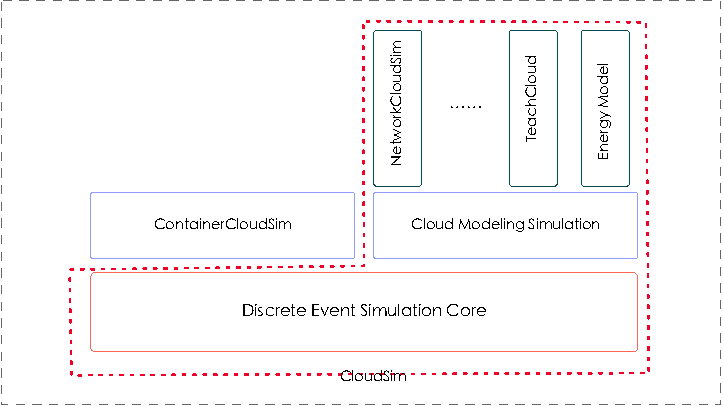
\includegraphics{container-cloudsim}
	\caption{ContainerCloudSim与CloudSim生态圈}
	\label{fig:xfig1}
\end{figure}
集成ContainerCloudSim的CloudSim-4.0云平台模拟器已完整支持容器云的仿真,新的版本具有如下几个特点:
\begin{enumerate}[(1)]
	\item 支持数据中心大规模云计算建模和仿真。
	\item 支持服务器虚拟化和主机的建模仿真,定制虚拟机调度策略。
	\item 支持容器应用程序的建模和仿真。
	\item 支持能量感知的计算资源建模和仿真。
	\item 支持网络拓扑结构和消息传递应用建模和仿真。
	\item 支持动态插入元素、停止和恢复的模拟。
	\item 支持混合云的建模和仿真。
\end{enumerate}

在ContainerCloudSim部分,提供容器、VMs、Host、数据中心资源包括CPU、内存和存储的管理功能,实现动态监控系统性、控制容器内应用的执行以及给容器提供虚拟机。容器的模拟器要能给研究人员提供容器调度方案间的对比,容器调度策略决定容器如何被调度到虚拟机上,以及各种调度算法之间的对比和评测。算法的能耗问题也是容器模拟器应该关注的重点,可以提供各种算法的能耗度量,容器的合并和迁移也是模拟器的一大功能。最后,模拟器要能够支持容器的扩展性,在CaaS容器环境中,容器的数量是远远多于虚拟机的。ContainerCloudSim是在CloudSim基础上开发而来,也是一个分层的架构,整体架构如下所示。
\begin{figure}[H] % use float package if you want it here
	\centering
	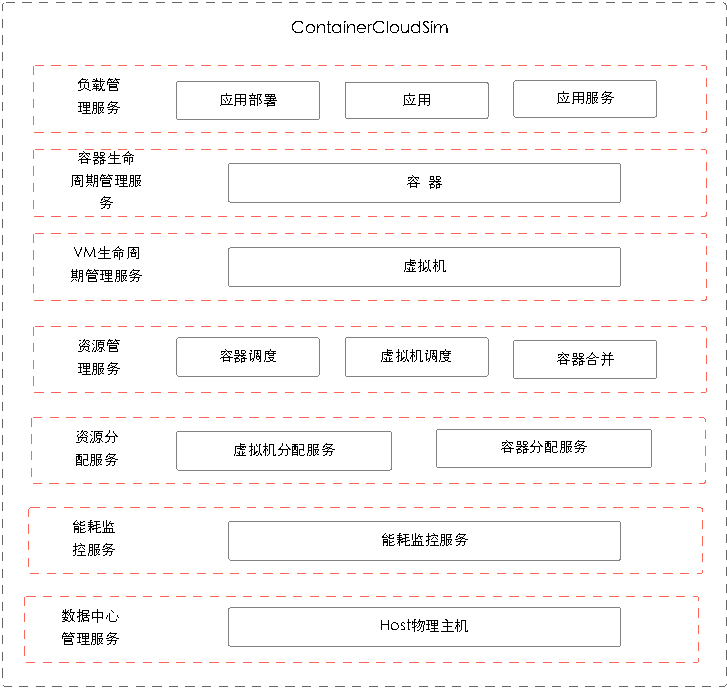
\includegraphics{containercloudsim-layer}
	\caption{ContainerCloudSim分层架构图}
	\label{fig:xfig1}
\end{figure}
从底至上依次分为数据中心管理服务、能耗监控服务、资源分配服务、资源管理服务、虚拟机生命周期管理服务、容器生命周期管理服务和负载管理服务等。每个层次的大致作用如下:
\begin{enumerate}
	\item 负载管理服务层关注于客户端应用的注册、部署、调度、应用层级的性能以及应用健康监控。
	\item 容器生命周期服务管理层负责容器生命周期管理,包括创建容器、注册容器到系统中、启动、停止、重启、从一个主机迁移到另一个主机以及容器销毁。除此之外,还负责执行和管理在容器中任务,监控任务资源利用率。
	\item 虚拟机生命周期管理服务层负责虚拟机的管理包括创建、启动、停止、重启、销毁、迁移以及资源利用率监控。
	\item 资源管理服务层负责容器在满足资源需求和软件环境的虚拟机上创建,虚拟机在满足资源需求的主机上创建,由容器调度、虚拟机调度和合并服务构成。容器调度根据容器调度策略调度容器到虚拟机、虚拟机调度根据虚拟机调度策略调度虚拟机到主机,合并策略通过合并容器减少主机需求,最小化资源碎片。
	\item 资源分配层服务管理虚拟机和容器的资源分配,由容器分配服务和虚拟机分配服务构成。容器分配服务负责虚拟机资源分配给容器,虚拟机分配服务负责主机资源分配给虚拟机。
	\item 能耗监控服务负责数据中心主机能耗监控,构建必要的能耗模型。
	\item 数据中心管理服务负责管理数据中心资源,主机开关机以及监控资源利用率。
\end{enumerate}
至此,ContainerCloudSim容器云仿真平台介绍完毕,具体的仿真执行流程具体的实现可以参见其源代码。

\subsection{MRWS资源利用率测试}






























